
至此，
关于同伦 (7.2.298.1) 及其带 $s$ 参数版本的讨论已完成。
下面讨论同伦 (7.2.298.2)
及其带 $s$ 参数版本。

回顾定理~\ref{thm:4-6-44} 的证明。
引理~\ref{lem:4-6-45} 指出，
若适当选择一族殆复结构，
用于定义
$\mathfrak f^{\psi\circ\phi_{1,s_0}}$
的模空间，
就与用于定义
$\mathfrak f^\psi\circ\mathfrak f^{\phi_{1,s_0}}$
的模空间相同。
换言之，按照第 7.2.10 小节所述方式，
在两种不同的殆复结构族、
扰动等选择之间插值，
即可得到同伦 (7.2.298.2)。
因此有下述结果。

\begin{lemma}{7.2.327}\label{lem:7-2-327}
存在滤过 $A_{n',K'}$ 代数
\[
C_b^{s=s_0}([0,1]_r\times L'_1,(\lambda_0,\lambda'_1)),
\]
以及滤过 $A_{n',K'}$ 同态
\[
\operatorname{Incl}_r\colon
C(L'_1,\lambda'_1)
\longrightarrow
C_b^{s=s_0}([0,1]_r\times L'_1,
(\lambda_0,\lambda'_1))
\]
和满足 (7.2.175) 的
$\operatorname{Eval}_{r=r_0}$，
另有滤过 $A_{n,K}$ 同态
\[
\mathcal F_b^{s=s_0}\colon
C(L_0,\lambda_0)
\longrightarrow
C_b^{s=s_0}([0,1]_r\times L'_1,
(\lambda_0,\lambda'_1)),
\]
使图式~\ref{diag:7-2-20} 交换。

\par\medskip\noindent\begin{minipage}{\textwidth}
\centering
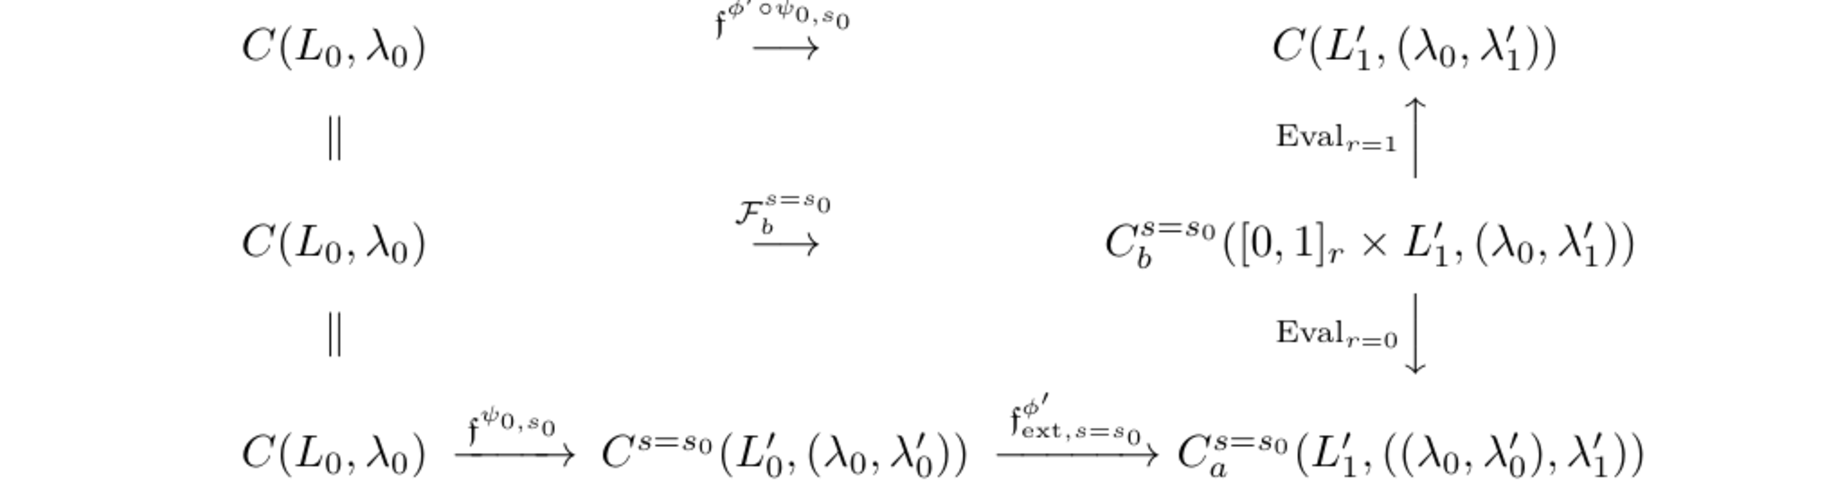
\includegraphics[width=\textwidth]{chapters/ch07-transversality/figures/phys-566-diagram-7-2-20-math-only-crop.png}
\par{\renewcommand{\thefigure}{7.2.20}\refstepcounter{figure}
\normalfont\bfseries 图式~\thefigure\label{diag:7-2-20}}
\end{minipage}\par\medskip
\end{lemma}

同理可证明如下带 $s$ 参数的版本。

\begin{lemma}{7.2.328}\label{lem:7-2-328}
存在滤过 $A_{n',K'}$ 代数
\[
C_b([0,1]^2\times L'_1,(\lambda_0,\lambda'_1)),
\]
滤过 $A_{n',K'}$ 同态
\[
\operatorname{Incl}\colon
C(L'_1,\lambda'_1)
\longrightarrow
C_b([0,1]^2\times L'_1,
(\lambda_0,\lambda'_1))
\]
和满足 (7.2.189) 的
$\operatorname{Eval}_{s=s_0}$、
$\operatorname{Eval}_{r=r_0}$，
以及滤过 $A_{n,K}$ 同态
\[
\mathfrak H_b\colon
C(L_0,\lambda_0)
\longrightarrow
C_b([0,1]^2\times L'_1,
(\lambda_0,\lambda'_1)),
\]
使
\[
\operatorname{Eval}_{s=s_0}\circ\mathfrak H_b
=\mathcal F_b^{s=s_0},
\]
且图式~\ref{diag:7-2-21} 交换。

\par\medskip\noindent\begin{minipage}{\textwidth}
\centering
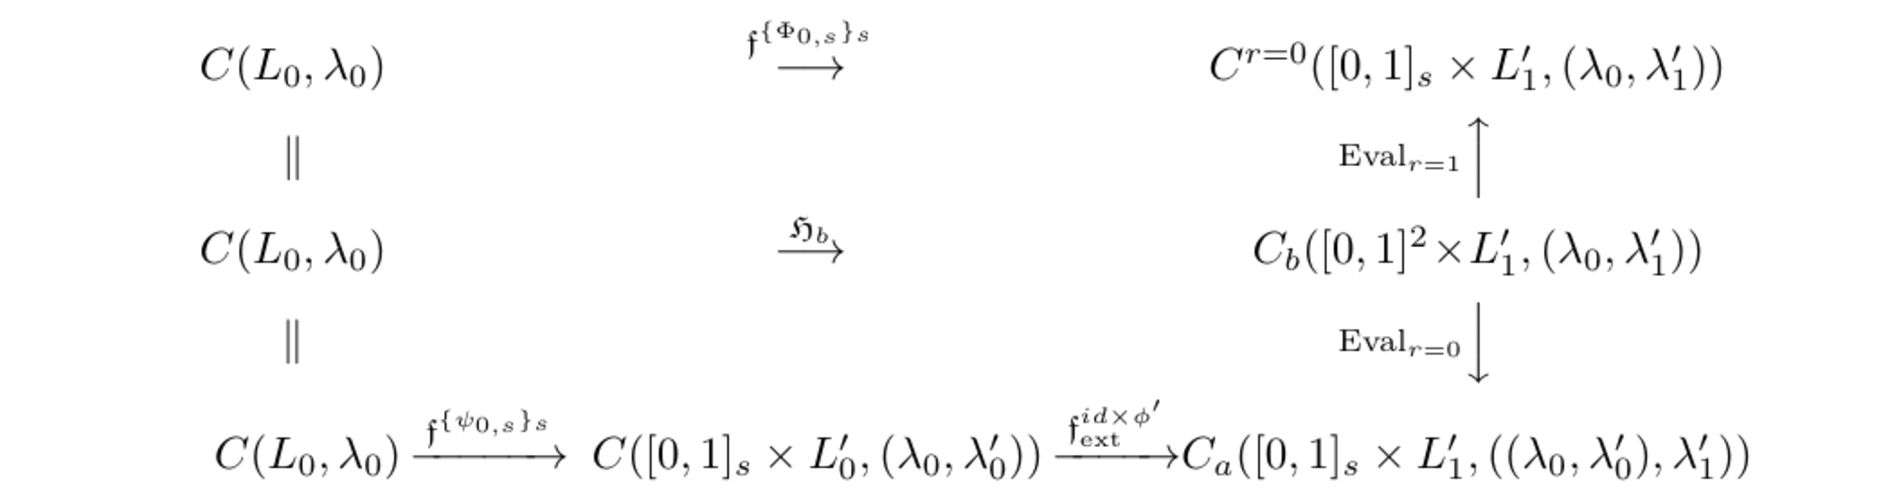
\includegraphics[width=\textwidth]{chapters/ch07-transversality/figures/phys-567-diagram-7-2-21-math-final-crop.png}
\par{\renewcommand{\thefigure}{7.2.21}\refstepcounter{figure}
\normalfont\bfseries 图式~\thefigure\label{diag:7-2-21}}
\end{minipage}\par\medskip
\end{lemma}

注意 $\Phi_{0,s}=\phi'\circ\psi_{0,s}$。\translatornote{原书图式 7.2.21 右上对象标作
$C^{r=0}([0,1]_s\times L'_1,(\lambda_0,\lambda'_1))$，
但从中央对象指向它的箭头标作
$\operatorname{Eval}_{r=1}$；
此处保留原图标注，待后文核对端面模型。}
因此，引理~\ref{lem:7-2-328}
是引理~\ref{lem:7-2-327}
的参数化版本。
其证明与引理~\ref{lem:7-2-285}
的证明相同。
我们所用的复形
$C_b([0,1]^2\times L'_1,(\lambda_0,\lambda'_1))$
是
$S([0,1]^2\times L'_1)$
的子复形，
后者已在引理~\ref{lem:7-2-285}
的证明中构造。
至此完成对 (7.2.280.1) 的讨论。

\begin{remark}{7.2.329}\label{rem:7-2-329}
这里用到一个事实：
$\mathfrak f^{\operatorname{id}\times\phi'}_{\mathrm{ext}}$
由模空间 (7.2.302) 的虚基本链
所定义的对应关系给出。
见注~\ref{rem:7-2-303}(2)。
\end{remark}
